\documentclass{article}
\usepackage[UTF8]{ctex}
\usepackage{sectsty}
\usepackage{amssymb,amsmath,amsthm,mathrsfs,graphicx}
\usepackage{tikz}
\usepackage{needspace}
\setlength{\emergencystretch}{2em}
\clubpenalty=10000\widowpenalty=10000
\title{泛函分析作业第四周}
\author{张溢致 2024011936}
\date{}
\begin{document}
\maketitle

\par\medskip\Needspace{5\baselineskip}\noindent 1. (i) 证明 $(C[0,1],\|\cdot\|_\infty)$ 是 Banach 空间。该空间可分吗？说明理由。

(ii) 证明 $\{f\in C[0,1]:\|f\|_\infty\le1\}$ 是有界闭集，但非完全有界。

(iii) 设 $A\subset C[0,1]$。证明 $A$ 完全有界当且仅当 $A$ 作为连续函数族一致有界且等度连续。

(iv) 设 $A\subset C[0,1]$。证明 $A$ 紧当且仅当 $A$ 闭且 $A$ 作为连续函数族一致有界且等度连续。


\par\Needspace{4\baselineskip}\noindent\textbf{解：}\par\nopagebreak[4]



(i) 设 $(f_n)$ 是一致范数下的 Cauchy 列。对每个 $x\in[0,1]$，由
\[
|f_n(x)-f_m(x)|\le\|f_n-f_m\|_\infty
\]
知 $(f_n(x))$ 是数域中的 Cauchy 列，故可定义 $f(x)=\lim_n f_n(x)$。任给 $\varepsilon>0$，取 $N$ 使得 $n,m\ge N$ 时 $\|f_n-f_m\|_\infty<\varepsilon/2$。固定 $n\ge N$，令 $m\to\infty$，得到对所有 $x$ 都有 $|f_n(x)-f(x)|\le\varepsilon/2$，所以 $f_n\to f$ 一致收敛。连续函数的一致极限连续，故 $f\in C[0,1]$。于是该空间完备。

该空间可分。令 $D$ 为所有如下折线函数构成的集合：对某个 $n\ge1$，节点为 $j/n$（$0\le j\le n$），节点值为有理数，相邻节点间作线性插值。复值情形将节点值改为实部、虚部均为有理数的数。每个 $n$ 对应的节点值集合可数，故 $D$ 可数。任给 $f\in C[0,1]$ 和 $\varepsilon>0$，由一致连续性可选 $n$ 使 $|x-y|\le1/n$ 时 $|f(x)-f(y)|<\varepsilon/2$。在各节点选择有理近似值 $q_j$，使 $|q_j-f(j/n)|<\varepsilon/2$，并令 $g\in D$ 为相应折线。在每个小区间上，把 $g(x)-f(x)$ 写成两个端点误差的凸组合，即得 $|g(x)-f(x)|<\varepsilon$。故 $D$ 稠密。

(ii) 记 $B=\{f:\|f\|_\infty\le1\}$。显然 $B$ 有界。若 $f_n\in B$ 且 $f_n\to f$ 一致收敛，则对每个 $x$ 有 $|f(x)|=\lim_n|f_n(x)|\le1$，所以 $f\in B$，故 $B$ 闭。

令 $f_n(x)=x^{2^n}$，则 $f_n\in B$。若 $m>n$，取 $x_n=2^{-1/2^n}$，有
\[
f_n(x_n)=\frac12,\qquad f_m(x_n)=2^{-2^{m-n}}\le\frac14,
\]
从而 $\|f_n-f_m\|_\infty\ge1/4$。任一半径为 $1/10$ 的开球至多包含一个 $f_n$，否则球内两函数的距离小于 $1/5$。所以有限个这样的球不能覆盖 $B$，即 $B$ 非完全有界。

(iii) 若 $A=\varnothing$，结论显然。以下设 $A\ne\varnothing$。先设 $A$ 完全有界。取有限个函数 $g_1,\ldots,g_N\in C[0,1]$，使每个 $f\in A$ 都满足某个 $\|f-g_j\|_\infty<1$。于是
\[
\|f\|_\infty\le1+\max_{1\le j\le N}\|g_j\|_\infty,
\]
故 $A$ 一致有界。任给 $\varepsilon>0$，再取有限个半径为 $\varepsilon/3$ 的球覆盖 $A$，记球心为 $h_1,\ldots,h_M$。由这些函数一致连续，可选同一个 $\delta>0$，使 $|x-y|<\delta$ 时对所有 $j$ 有 $|h_j(x)-h_j(y)|<\varepsilon/3$。对任意 $f\in A$，选 $j$ 使 $\|f-h_j\|_\infty<\varepsilon/3$，则
\[
|f(x)-f(y)|\le2\|f-h_j\|_\infty+|h_j(x)-h_j(y)|<\varepsilon.
\]
所以 $A$ 等度连续。

反之，设 $A$ 一致有界且等度连续。紧区间上的等度连续性给出统一控制：任给 $\eta>0$，存在 $\delta>0$，使 $|x-y|<\delta$ 时对所有 $f\in A$ 都有 $|f(x)-f(y)|<\eta$。若采用逐点定义，可在每个点先以 $\eta/2$ 取得一个控制邻域，再选取半径减半的有限子覆盖，并取这些半径的最小值的一半，即得上述统一控制。

现给定 $\varepsilon>0$，取 $\eta=\varepsilon/4$，并选网格 $0=t_0<\cdots<t_k=1$，使网格间距小于相应的 $\delta$。设 $\|f\|_\infty\le M$ 对所有 $f\in A$ 成立。闭圆盘 $\{z:|z|\le M\}$（实值时为闭区间）可由有限个半径为 $\eta$ 的开球覆盖。依次记录各节点值 $f(t_i)$ 所属的一个球，只有有限种记录。每种实际出现的记录选一个代表函数 $g\in A$。若 $f$ 与 $g$ 的记录相同，则 $|f(t_i)-g(t_i)|<2\eta$。任给 $x$，选相邻节点 $t_i$ 使 $|x-t_i|<\delta$，有
\[
|f(x)-g(x)|\le|f(x)-f(t_i)|+|f(t_i)-g(t_i)|+|g(t_i)-g(x)|<4\eta=\varepsilon.
\]
这些有限个代表构成 $A$ 的 $\varepsilon$-网。因此 $A$ 完全有界。

(iv) 若 $A$ 紧，则 $A$ 闭且完全有界，由 (iii) 得一致有界和等度连续。反之，若 $A$ 闭、一致有界且等度连续，由 (i) 知 $A$ 完备，由 (iii) 知 $A$ 完全有界。由度量空间中“紧等价于完备且完全有界”，得到 $A$ 紧。


\par\medskip\Needspace{5\baselineskip}\noindent 2. 在 $C([0,1])$ 上定义
\[
\|f\|_1:=\int_0^1|f(x)|\,dx.
\]
证明 $\|\cdot\|_1$ 与 $\|\cdot\|_\infty$ 不等价。


\par\Needspace{4\baselineskip}\noindent\textbf{解：}\par\nopagebreak[4]



对任意 $f\in C[0,1]$，有 $\|f\|_1\le\|f\|_\infty$。令
\[
f_n(x)=\max\{1-nx,0\}.
\]
则 $f_n\in C[0,1]$，且
\[
\|f_n\|_\infty=1,\qquad
\|f_n\|_1=\int_0^{1/n}(1-nx)\,dx=\frac1{2n}.
\]
若两范数等价，则存在与 $f$ 无关的 $C>0$，使 $\|f\|_\infty\le C\|f\|_1$。代入 $f_n$ 得 $1\le C/(2n)$，令 $n\to\infty$ 即得矛盾。故两范数不等价。


\par\medskip\Needspace{5\baselineskip}\noindent 3. 设 $X$ 是非空集合。定义 $B(X)$ 为 $X$ 上所有有界函数构成的线性空间。对 $f\in B(X)$ 定义
\[
\|f\|_\infty:=\sup\{|f(x)|:x\in X\}.
\]
证明 $\|\cdot\|_\infty$ 是 $B(X)$ 上的范数，且 $B(X)$ 在此范数下为 Banach 空间。给出 $B(X)$ 可分的充要条件。


\par\Needspace{4\baselineskip}\noindent\textbf{解：}\par\nopagebreak[4]



非负性及绝对齐次性直接由上确界的定义得到。若 $\|f\|_\infty=0$，则 $f(x)=0$ 对所有 $x$ 成立；反之显然。又
\[
|f(x)+g(x)|\le|f(x)|+|g(x)|\le\|f\|_\infty+\|g\|_\infty,
\]
取上确界得三角不等式。因此 $\|\cdot\|_\infty$ 是范数。

设 $(f_n)$ 为 $B(X)$ 中的 Cauchy 列。逐点定义 $f(x)=\lim_n f_n(x)$。任给 $\varepsilon>0$，取 $N$ 使 $n,m\ge N$ 时 $\|f_n-f_m\|_\infty<\varepsilon/2$。令 $m\to\infty$ 得 $|f_n(x)-f(x)|\le\varepsilon/2$，对全部 $x$ 同时成立。特别地，取一次 $\varepsilon=2$，得到 $|f(x)|\le|f_N(x)|+1$，所以 $f$ 有界。再由任意的 $\varepsilon$ 知 $\|f_n-f\|_\infty\to0$，故 $B(X)$ 完备。

$B(X)$ 可分的充要条件是 $X$ 有限。若 $X$ 有限，则 $B(X)$ 与有限维坐标空间等距同构，取有理坐标即可得到可数稠密集。

若 $X$ 无限，选互异点 $x_1,x_2,\ldots\in X$。对每个 $S\subset\mathbb N$，定义 $f_S=\mathbf1_{\{x_n:n\in S\}}$。若 $S\ne T$，则 $\|f_S-f_T\|_\infty=1$，故得到不可数个两两距离为 $1$ 的函数。可分度量空间中这样的集合必可数：若 $D$ 是可数稠密集，则每个半径为 $1/3$ 的球 $B(f_S,1/3)$ 都包含 $D$ 中某点，而这些球两两不交，因此球的个数至多可数。矛盾，故 $B(X)$ 不可分。


\par\medskip\Needspace{5\baselineskip}\noindent 4. 设 $(X,d)$ 是度量空间，定义 $C(X)$ 的子空间 $C_b(X):=C(X)\cap B(X)$。证明 $C_b(X)$ 是 $B(X)$ 的闭子空间，从而 $C_b(X)$ 为 Banach 空间。


\par\Needspace{4\baselineskip}\noindent\textbf{解：}\par\nopagebreak[4]



连续有界函数对加法和数乘封闭，故 $C_b(X)$ 是 $B(X)$ 的线性子空间。设 $f_n\in C_b(X)$，且 $\|f_n-f\|_\infty\to0$，其中 $f\in B(X)$。任取 $x_0\in X$ 和 $\varepsilon>0$，先固定 $n$ 使 $\|f-f_n\|_\infty<\varepsilon/3$，再由 $f_n$ 在 $x_0$ 连续，选 $\delta>0$ 使 $d(x,x_0)<\delta$ 时 $|f_n(x)-f_n(x_0)|<\varepsilon/3$。于是
\[
\begin{aligned}
|f(x)-f(x_0)|
\le{}&|f(x)-f_n(x)|\\
&+|f_n(x)-f_n(x_0)|\\
&+|f_n(x_0)-f(x_0)|\\
\le{}&2\|f-f_n\|_\infty+|f_n(x)-f_n(x_0)|\\
<{}&\varepsilon.
\end{aligned}
\]
故 $f$ 连续，从而 $f\in C_b(X)$，即 $C_b(X)$ 闭。由第 3 题 $B(X)$ 完备，而完备空间的闭子空间完备，故 $C_b(X)$ 为 Banach 空间。


\par\medskip\Needspace{5\baselineskip}\noindent 5. 设 $X$ 是一个线性空间，$p:X\to\mathbb R_+$ 是一个半范数。

1) 令 $Y:=\{x\in X:p(x)=0\}$，证明 $Y$ 是 $X$ 的线性子空间。

2) 在 $X$ 上定义关系 $\sim$ 为：$x\sim y$ 当且仅当 $p(x-y)=0$。证明 $\sim$ 是 $X$ 上的等价关系，且商空间 $X/Y$ 恰为 $X/{\sim}$。

3) 在 $X/Y$ 上定义 $\|\cdot\|$ 为 $\|\widetilde x\|:=p(x)$，证明 $\|\cdot\|$ 良定义，且其是 $X/Y$ 上的范数。


\par\Needspace{4\baselineskip}\noindent\textbf{解：}\par\nopagebreak[4]



1) 由半范数的齐次性，$p(0)=0$，故 $0\in Y$。若 $x,y\in Y$，$a,b$ 为标量，则
\[
0\le p(ax+by)\le |a|p(x)+|b|p(y)=0,
\]
所以 $ax+by\in Y$。因此 $Y$ 是线性子空间。

2) 自反性由 $p(x-x)=0$ 得到；对称性由 $p(y-x)=p(-(x-y))=p(x-y)$ 得到。若 $x\sim y$ 且 $y\sim z$，则
\[
p(x-z)\le p(x-y)+p(y-z)=0,
\]
故 $x\sim z$。所以这是等价关系。并且
\[
[x]_{\sim}=\{y:p(y-x)=0\}=\{y:y-x\in Y\}=x+Y,
\]
恰为商空间中的陪集，故 $X/Y=X/{\sim}$。

3) 若 $x+Y=x'+Y$，则 $p(x-x')=0$。由三角不等式，$p(x)\le p(x')+p(x-x')=p(x')$，交换 $x,x'$ 得反向不等式，故 $p(x)=p(x')$。因此范数定义与代表元无关。又
\[
\|[x]\|=0\iff p(x)=0\iff x\in Y\iff[x]=[0],
\]
而 $\|a[x]\|=p(ax)=|a|p(x)=|a|\|[x]\|$，以及
\[
\|[x]+[y]\|=p(x+y)\le p(x)+p(y)=\|[x]\|+\|[y]\|.
\]
故它是 $X/Y$ 上的范数。


\par\medskip\Needspace{5\baselineskip}\noindent 6. 定义 $p:\mathbb R^3\to\mathbb R_+$ 为 $p(x):=|x_3|$。

1) 证明 $p$ 是 $\mathbb R^3$ 上的半范数。

2) 确定 $Y=\{x\in\mathbb R^3:p(x)=0\}$。并按上题确定 $\mathbb R^3/Y$ 上的范数 $\|\cdot\|$。

3) 证明 n.l.s. $(\mathbb R^3/Y,\|\cdot\|)$ 与 $Z:=\{(0,0,z):z\in\mathbb R\}$（取欧式范数 $|\cdot|$）等距线性同构，即存在线性同构 $\varphi:\mathbb R^3/Y\to Z$ 使得 $|\varphi(\widetilde x)|=\|\widetilde x\|$。


\par\Needspace{4\baselineskip}\noindent\textbf{解：}\par\nopagebreak[4]



1) 对 $x,y\in\mathbb R^3$ 和 $\lambda\in\mathbb R$，有
\[
p(\lambda x)=|\lambda x_3|=|\lambda|p(x),\qquad
p(x+y)=|x_3+y_3|\le p(x)+p(y).
\]
故 $p$ 是半范数。

2) $Y=\{(x_1,x_2,0):x_1,x_2\in\mathbb R\}$。由第 5 题，商空间的范数为
\[
\|[(x_1,x_2,x_3)]\|=|x_3|.
\]

3) 定义 $\varphi([(x_1,x_2,x_3)])=(0,0,x_3)$。同一陪集中的向量第三个坐标相同，故定义良好。该映射线性、满射，且核只有零陪集，所以是线性同构。最后
\[
|\varphi([x])|=|(0,0,x_3)|=|x_3|=\|[x]\|,
\]
故为等距线性同构。


\par\medskip\Needspace{5\baselineskip}\noindent 7. 设 $X$ 为线性空间，$d$ 为 $X$ 上的一个度量且满足
\begin{equation}
\begin{aligned}
d(x+z,y+z)&=d(x,y)\quad(\forall x,y,z\in X);\\
d(\lambda x,\lambda y)&=|\lambda|d(x,y).
\end{aligned}\tag{1}\label{eq:metric}
\end{equation}
定义 $\|\cdot\|:X\to\mathbb R_+$ 为 $\|x\|:=d(x,0)$。证明 $\|\cdot\|$ 是 $X$ 上的一个范数。


\par\Needspace{4\baselineskip}\noindent\textbf{解：}\par\nopagebreak[4]



由 $d$ 是度量，$\|x\|=d(x,0)\ge0$，且 $\|x\|=0$ 当且仅当 $x=0$。由第二个条件，
\[
\|\lambda x\|=d(\lambda x,\lambda0)=|\lambda|d(x,0)=|\lambda|\|x\|.
\]
再用三角不等式及平移不变性，得到
\[
\|x+y\|=d(x+y,0)\le d(x+y,y)+d(y,0)=d(x,0)+d(y,0).
\]
所以 $\|\cdot\|$ 是范数。


\par\medskip\Needspace{5\baselineskip}\noindent 8. 设 $0<p<1$。

1) 定义 $\|\cdot\|_p:\mathbb R^n\to\mathbb R_+$ 为
\[
\|x\|_p:=\left(\sum_{j=1}^n|x_j|^p\right)^{1/p}.
\]
证明 $\|\cdot\|_p$ 不是 $\mathbb R^n$ 上的范数。

2) 定义 $d_p:\mathbb R^n\times\mathbb R^n\to\mathbb R_+$ 为
\[
d_p(x,y):=\sum_{j=1}^n|x_j-y_j|^p.
\]
证明 $d_p$ 是 $\mathbb R^n$ 上的度量，且 $(\mathbb R^n,d_p)$ 完备。

3) 证明 $d_p$ 满足 (1) 中的第一条但是不满足第二条。

4) 画出单位球
\[
B:=\{x\in\mathbb R^2:d_p(x,0)\le1\}
\]
的图形。


\par\Needspace{4\baselineskip}\noindent\textbf{解：}\par\nopagebreak[4]



1) 当 $n\ge2$ 时，取前两个标准基向量 $e_1,e_2$，有
\[
\|e_1\|_p=\|e_2\|_p=1,\qquad
\|e_1+e_2\|_p=2^{1/p}>2.
\]
故三角不等式不成立，它不是范数。需要指出，原题此结论须补充 $n\ge2$；若 $n=1$，则 $\|x\|_p=|x|$，确为范数。

2) 先证对 $a,b\ge0$ 有 $(a+b)^p\le a^p+b^p$。当 $a+b>0$ 时，令 $t=a/(a+b)$，由 $0<p<1$ 知 $t^p\ge t$、$(1-t)^p\ge1-t$，所以
\[
a^p+b^p=(a+b)^p\bigl(t^p+(1-t)^p\bigr)\ge(a+b)^p.
\]
$a=b=0$ 时也成立。因此对实数 $u,v$，$|u+v|^p\le|u|^p+|v|^p$，从而
\[
d_p(x,z)\le\sum_{j=1}^n\bigl(|x_j-y_j|^p+|y_j-z_j|^p\bigr)=d_p(x,y)+d_p(y,z).
\]
非负性、对称性及 $d_p(x,y)=0\iff x=y$ 均直接成立，故 $d_p$ 是度量。

若 $(x^{(k)})$ 是 $d_p$-Cauchy 列，则对每个 $j$，
\[
|x_j^{(k)}-x_j^{(l)}|^p\le d_p(x^{(k)},x^{(l)})\to0,
\]
所以存在实数 $x_j$ 使 $x_j^{(k)}\to x_j$。令 $x=(x_1,\ldots,x_n)$，由有限项求和得 $d_p(x^{(k)},x)\to0$。所以该度量空间完备。

3) 直接有 $d_p(x+z,y+z)=d_p(x,y)$。但
\[
d_p(\lambda x,\lambda y)=|\lambda|^p d_p(x,y).
\]
取 $x\ne y$ 和 $\lambda=2$，因 $2^p\ne2$，知它不满足 (1) 的第二条。

\par\medskip\noindent\begin{minipage}{\linewidth}
4) 单位球为 $B=\{(x,y):|x|^p+|y|^p\le1\}$，关于两个坐标轴对称。在第一象限，边界为
\[
y=(1-x^p)^{1/p},\qquad0\le x\le1,
\]
单位球是该曲线与坐标轴围成的闭区域，再关于两轴反射。边界经过 $(\pm1,0),(0,\pm1)$，并向原点方向凹入；例如 $(1,0),(0,1)\in B$，但它们的中点不在 $B$，因为 $2(1/2)^p>1$。下图给出 $p=1/2$ 的代表图形，其他 $0<p<1$ 按上述边界公式作图。
\begin{center}
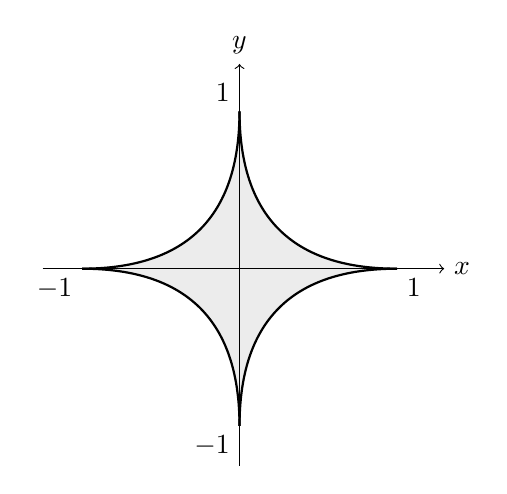
\begin{tikzpicture}[scale=2]
\fill[gray!15] plot[domain=0:1,samples=70] ({(1-\x)^2},{\x^2}) -- plot[domain=0:1,samples=70] ({-\x^2},{(1-\x)^2}) -- plot[domain=0:1,samples=70] ({-(1-\x)^2},{-\x^2}) -- plot[domain=0:1,samples=70] ({\x^2},{-(1-\x)^2}) -- cycle;
\draw[->] (-1.25,0)--(1.3,0) node[right] {$x$};
\draw[->] (0,-1.25)--(0,1.3) node[above] {$y$};
\draw[thick] plot[domain=0:1,samples=70] ({(1-\x)^2},{\x^2});
\draw[thick] plot[domain=0:1,samples=70] ({-(1-\x)^2},{\x^2});
\draw[thick] plot[domain=0:1,samples=70] ({-(1-\x)^2},{-\x^2});
\draw[thick] plot[domain=0:1,samples=70] ({(1-\x)^2},{-\x^2});
\node[below right] at (1,0) {$1$};\node[below left] at (-1,0) {$-1$};
\node[above left] at (0,1) {$1$};\node[below left] at (0,-1) {$-1$};
\end{tikzpicture}
\end{center}
\end{minipage}


\end{document}
